\documentclass[openany]{book}
\title{Estadística 1 - Material de apoyo}
\author{David Gabriel Corzo Mcmath}
\date{2020-01-07}

\usepackage[margin = 1in]{geometry}
\usepackage{graphicx}
\usepackage{fontenc}
\usepackage[spanish]{babel}
\usepackage{amsmath}
\usepackage{amsthm}
\usepackage{amssymb}
\usepackage[utf8]{inputenc}
\usepackage{enumitem}
\usepackage{mathtools}
\usepackage{fancyhdr}
\usepackage{lipsum}
\usepackage{sectsty}
\usepackage{titlesec}
\usepackage{tikz}
\usepackage{hyperref}
\usepackage{longtable}

\pagestyle{plain}

\begin{document}
\maketitle
\tableofcontents

% Here the document starts

%%%%%%%%%%%%%%%%%%%%%%%%%%%%%%%%%%%%%%%%%%%%%%%%%%%%%%%%%%%%%%%%%%%%%%%%%%%%%%%%%%%%%%%%%%%%%%%%

\part{ Examenes Cortos }

\chapter{ Examen corto \#01}
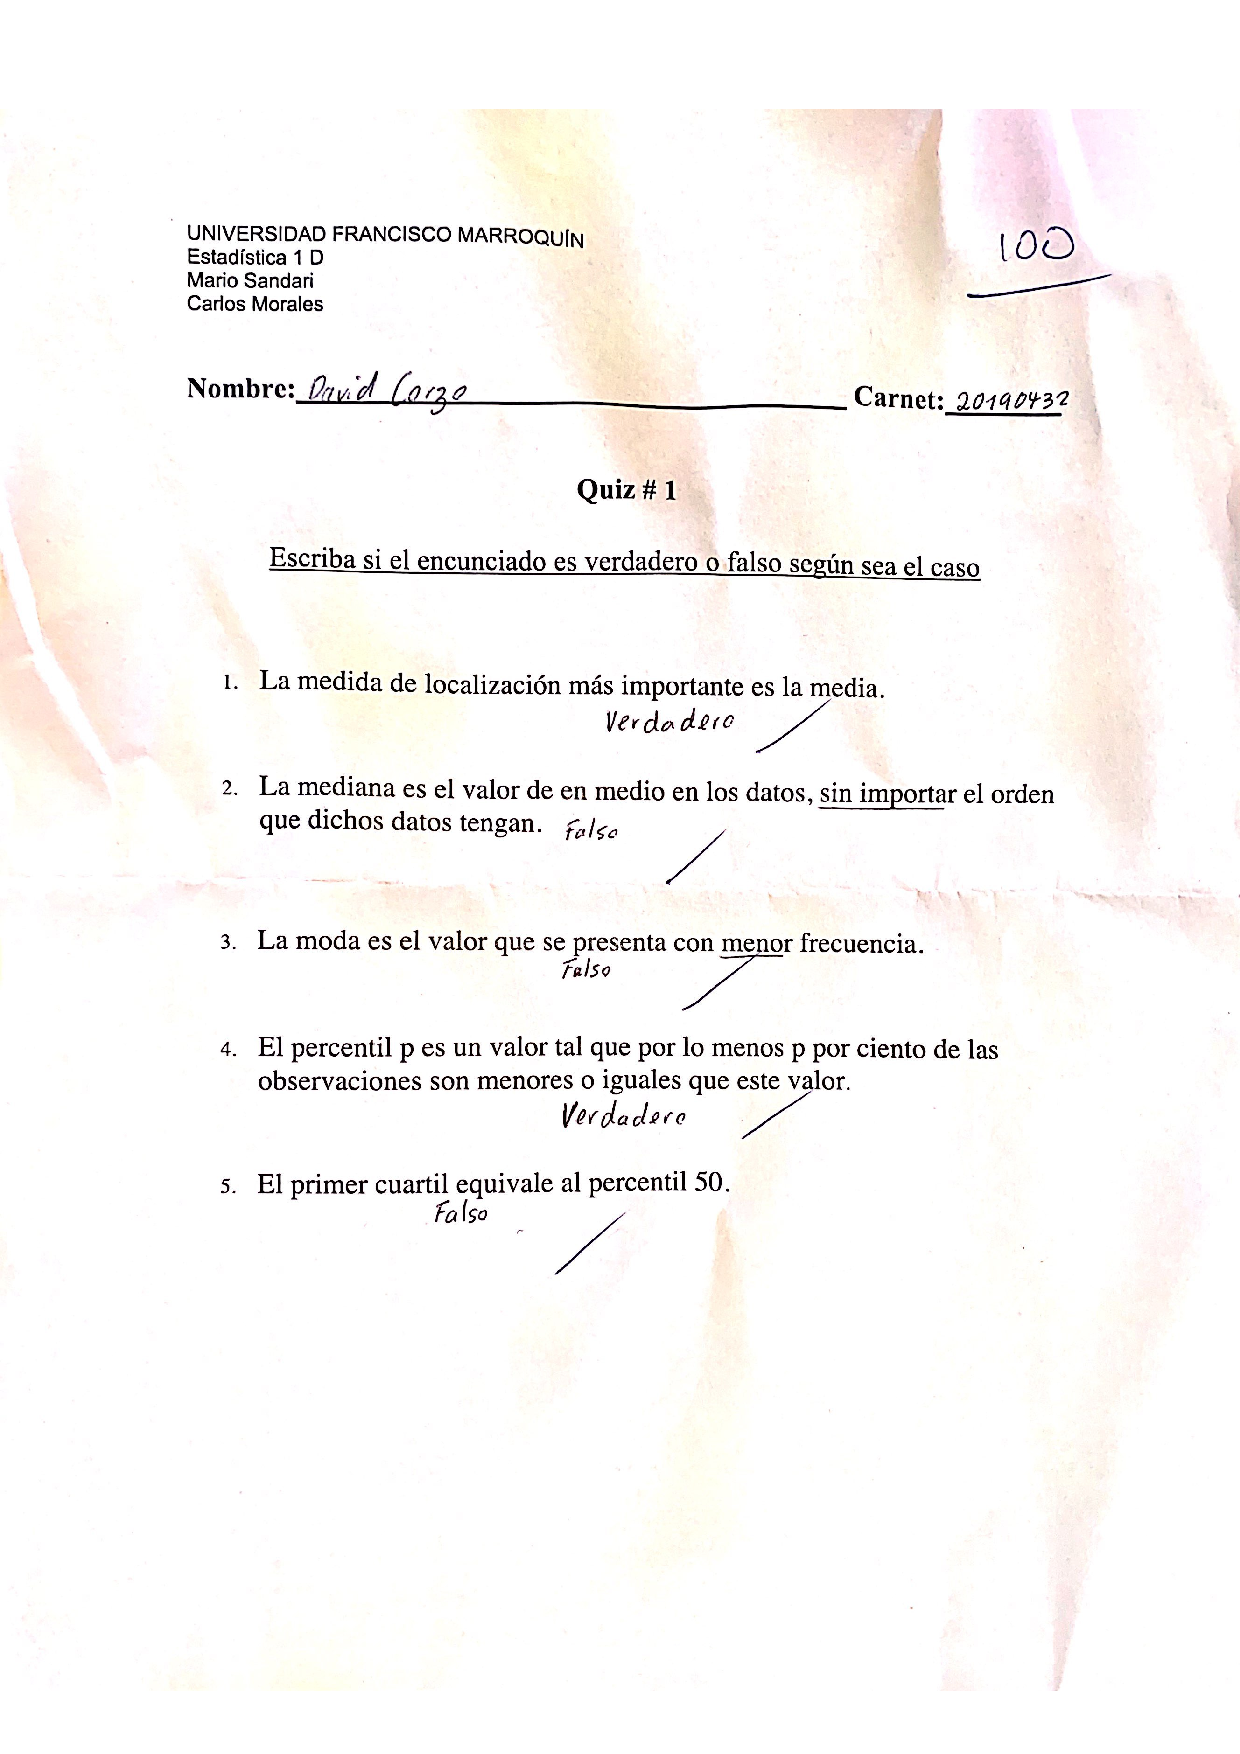
\includepdf[pages=-,pagecommand={\thispagestyle{plain}}]{\detokenize{pdf/EC_01_ESTADISTICA.pdf}} 

%%%%%%%%%%%%%%%%%%%%%%%%%%%%%%%%%%%%%%%%%%%%%%%%%%%%%%%%%%%%%%%%%%%%%%%%%%%%%%%%%%%%%%%%%%%%%%%%

% Here the document ends

\end{document}
